%% For double-blind review submission, w/o CCS and ACM Reference (max submission space)
\documentclass[sigplan,10pt,nonacm]{acmart}
\settopmatter{printfolios}
%% For double-blind review submission, w/ CCS and ACM Reference
%\documentclass[sigplan,review,anonymous]{acmart}\settopmatter{printfolios=true}
%% For single-blind review submission, w/o CCS and ACM Reference (max submission space)
%\documentclass[sigplan,review]{acmart}\settopmatter{printfolios=true,printccs=false,printacmref=false}
%% For single-blind review submission, w/ CCS and ACM Reference
%\documentclass[sigplan,review]{acmart}\settopmatter{printfolios=true}
%% For final camera-ready submission, w/ required CCS and ACM Reference
%\documentclass[sigplan]{acmart}\settopmatter{}


%% Conference information
%% Supplied to authors by publisher for camera-ready submission;
%% use defaults for review submission.
\acmConference[VEE'20]{ACM SIGPLAN/SIGOPS International Conference on Virtual Execution Environments}{March 17, 2020}{Lausanne, Switzerland}
\acmYear{2020}
\acmISBN{} % \acmISBN{978-x-xxxx-xxxx-x/YY/MM}
\acmDOI{} % \acmDOI{10.1145/nnnnnnn.nnnnnnn}
\startPage{1}

%% Copyright information
%% Supplied to authors (based on authors' rights management selection;
%% see authors.acm.org) by publisher for camera-ready submission;
%% use 'none' for review submission.
\setcopyright{none}
%\setcopyright{acmcopyright}
%\setcopyright{acmlicensed}
%\setcopyright{rightsretained}
%\copyrightyear{2018}           %% If different from \acmYear

%% Bibliography style
\bibliographystyle{ACM-Reference-Format}
%% Citation style
%\citestyle{acmauthoryear}  %% For author/year citations
\citestyle{acmnumeric}     %% For numeric citations
\setcitestyle{nosort}      %% With 'acmnumeric', to disable automatic
                            %% sorting of references within a single citation;
                            %% e.g., \cite{Smith99,Carpenter05,Baker12}
                            %% rendered as [14,5,2] rather than [2,5,14].
%\setcitesyle{nocompress}   %% With 'acmnumeric', to disable automatic
                            %% compression of sequential references within a
                            %% single citation;
                            %% e.g., \cite{Baker12,Baker14,Baker16}
                            %% rendered as [2,3,4] rather than [2-4].


%%%%%%%%%%%%%%%%%%%%%%%%%%%%%%%%%%%%%%%%%%%%%%%%%%%%%%%%%%%%%%%%%%%%%%
%% Note: Authors migrating a paper from traditional SIGPLAN
%% proceedings format to PACMPL format must update the
%% '\documentclass' and topmatter commands above; see
%% 'acmart-pacmpl-template.tex'.
%%%%%%%%%%%%%%%%%%%%%%%%%%%%%%%%%%%%%%%%%%%%%%%%%%%%%%%%%%%%%%%%%%%%%%


%% Some recommended packages.
\usepackage{booktabs}   %% For formal tables:
                        %% http://ctan.org/pkg/booktabs
\usepackage{subcaption} %% For complex figures with subfigures/subcaptions
                        %% http://ctan.org/pkg/subcaption
%\usepackage[tight,footnotesize]{subfigure}
\usepackage{caption}
\usepackage{subcaption}
\begin{document}

%% Title information
\title[]{CPU and Memory Over-commitment for HPC Cloud}         %% [Short Title] is optional;
                                        %% when present, will be used in
                                        %% header instead of Full Title.
%\titlenote{with title note}             %% \titlenote is optional;
                                        %% can be repeated if necessary;
                                        %% contents suppressed with 'anonymous'
%\subtitle{Subtitle}                     %% \subtitle is optional
%\subtitlenote{with subtitle note}       %% \subtitlenote is optional;
                                        %% can be repeated if necessary;
                                        %% contents suppressed with 'anonymous'


%% Author information
%% Contents and number of authors suppressed with 'anonymous'.
%% Each author should be introduced by \author, followed by
%% \authornote (optional), \orcid (optional), \affiliation, and
%% \email.
%% An author may have multiple affiliations and/or emails; repeat the
%% appropriate command.
%% Many elements are not rendered, but should be provided for metadata
%% extraction tools.

%% Author with single affiliation.
\author{Anonymized}
% \author{Xiaolong Cui}
% \affiliation{
%   %\position{HPC Engineer}
%   %\department{Office of the CTO}              %% \department is recommended
%   \institution{VMware, Inc.}            %% \institution is required
%   %\streetaddress{Street1 Address1}
%   \city{Boston}
%   %\state{California}
%   %\postcode{Post-Code1}
%   \country{USA}                    %% \country is recommended
% }
% \email{xiaolongc@vmware.com} 

% \author{Josh Simons}
% %\authornote{with author1 note}          %% \authornote is optional;
%                                         %% can be repeated if necessary
% %\orcid{nnnn-nnnn-nnnn-nnnn}             %% \orcid is optional
% \affiliation{
%   %\position{HPC Engineer}
%   %\department{Office of the CTO}              %% \department is recommended
%   \institution{VMware, Inc.}            %% \institution is required
%   %\streetaddress{Street1 Address1}
%   \city{Boston}
%   %\state{California}
%   %\postcode{Post-Code1}
%   \country{USA}                    %% \country is recommended
% }
% \email{simons@vmware.com}          %% \email is recommended

% %% Author with two affiliations and emails.
% \author{Na Zhang}
% %\authornote{with author1 note}          %% \authornote is optional;
%                                         %% can be repeated if necessary
% %\orcid{nnnn-nnnn-nnnn-nnnn}             %% \orcid is optional
% \affiliation{
%   %\position{HPC Engineer}
%   %\department{Office of the CTO}              %% \department is recommended
%   \institution{VMware, Inc.}            %% \institution is required
%   %\streetaddress{Street1 Address1}
%   \city{Boston}
%   %\state{California}
%   %\postcode{Post-Code1}
%   \country{USA}                    %% \country is recommended
% }
% \email{nz@vmware.com}  

%% Abstract
%% Note: \begin{abstract}...\end{abstract} environment must come
%% before \maketitle command
\begin{abstract}
With the concerted efforts from researchers in hardware, software, algorithm, and data management, HPC is moving towards extreme-scale, featuring a computing capability of quintillion ($10^{18}$) FLOPS. 
As we approach the new era of computing, however, several daunting scalability challenges remain to be conquered. Delivering extreme-scale performance will require a computing platform that supports billion-way parallelism, necessitating a dramatic increase in the number of computing, storage, and networking components. At such a large scale, failure would become a norm rather than an exception, driving the system to significantly lower efficiency with unprecedented amount of power consumption. %The frequency and diversity of failures,  as well as the challenge of power, call for rethinking of the fault tolerance problem. 

To tackle this challeng, we propose an adaptive and power-aware algorithm, referred to as Lazy Shadowing, as an efficient and scalable approach to achieve high-levels of resilience, through forward progress, in extreme-scale, failure-prone computing environments. 
Lazy Shadowing associates with each process a ``shadow" (process) that executes at a reduced rate, and opportunistically rolls forward each shadow to catch up with the its leading process during failure recovery.
%overlaps the recovery time after each failure with the time needed to roll forward the shadows to a consistent state.
Compared to existing fault tolerance methods, our approach can achieve 20\% energy saving with potential reduction in solution time at scale.


\end{abstract}


%% 2012 ACM Computing Classification System (CSS) concepts
%% Generate at 'http://dl.acm.org/ccs/ccs.cfm'.
%\begin{CCSXML}
%<concept>
%<concept_id>10011007.10011006.10011008</concept_id>
%<concept_desc>Software and its engineering~General programming languages</concept_desc>
%<concept_significance>500</concept_significance>
%</concept>
%<concept>
%<concept_id>10003456.10003457.10003521.10003525</concept_id>
%<concept_desc>Social and professional topics~History of programming languages</concept_desc>
%<concept_significance>300</concept_significance>
%</concept>
%</ccs2012>
%\end{CCSXML}

%\ccsdesc[500]{Software and its engineering~General programming languages}
%\ccsdesc[300]{Social and professional topics~History of programming languages}
%% End of generated code


%% Keywords
%% comma separated list
\keywords{Virtualization, HPC, Resource Management, Over-commitment, Multi-tenancy}  %% \keywords are mandatory in final camera-ready submission


%% \maketitle
%% Note: \maketitle command must come after title commands, author
%% commands, abstract environment, Computing Classification System
%% environment and commands, and keywords command.
\maketitle


\section{Introduction}
\label{sec:intro}
As our reliance on IT continues to increase, the complexity and urgency of the problems our society will face 
in the future drives us to build more powerful and accessible computer systems. Among the different types of 
computer systems, High Performance Computing (HPC) and Cloud Computing systems are the two most powerful ones. 
For both, the computing power attributes to the massive amount of parallelism, which is enabled by 
the massive amount of CPU cores, memory modules, communication devices, storage components, etc. 

Since CPU frequency flattened out in early 2000s, parallelism has become the ``golden rule" to boost performance. 
In HPC, Terascale performance was achieved in the late 90’s with fewer than 10,000 heavyweight single-core processors. 
A decade later, petascale performance required about ten times more processors with multiple cores on each processor. Nowadays, a race
is underway to build the world's first exascale machine to accelerate scientific discoveries and breakthroughs. It is 
projected that an exascale machine will achieve billion-way parallelism by using one million sockets each supporting 
1,000 cores~\cite{doe_ascr_exascale_2011,top_ten_2014}. 

Similar trend is happening in Cloud Computing. 
As the demand for Cloud Computing accelerates, cloud service providers  
will be faced with the need to expand their underlying infrastructure to ensure the expected levels of performance, reliability and cost-effectiveness. 
As a result, lots of large-scale data centers have been and are being built by IT companies
to exploit the power and economies of scale. 
For example, Google, Facebook, and Rackspace have hundreds of thousands 
of web servers in dedicated data centers to support their business. 

Unfortunately, several challenging issues come with the increase in system scale. As today's HPC and Cloud Computing systems grow to 
meet tomorrow's compute power demand, the behavior of the systems will be increasingly difficult to specify, predict and manage. 
This upward trend, in terms of scale and complexity, has a direct negative effect on the overall system reliability. 
%Even with the expected improvement in the reliability of future computing technology, the rate of system level failures will 
%dramatically increase with the number of components, possibly by several orders of magnitude. 
At the same time, the rapid 
growing power consumption, as a result of the increase in system components, is another major concern. 
%It is reported that 
%the power required to run the machines as well as cool them has become the largest cost factor in a large-scale system's operating 
%expenses.  
At future extreme-scale, failure would become a norm rather than an exception, 
driving the system to significantly lower efficiency with unprecedented amount of power consumption. 

\section{Problem Statement}

The system scale needed to address our future computing needs will come at the cost of increasing complexity, unpredictability, 
and operating expenses. As we approach future extreme-scale computing, two of the biggest challenges will be system resilience and power 
consumption, both being direct consequences of the dramatic increase in the number of system components~\cite{exa_challenge_2010,snir2014addressing}. 

Regardless of the reliability of individual component, the system level failure rate will continue to increase as the number of 
components increases, possibly by several orders of magnitude. It is projected that the Mean Time Between Failures (MTBF) of future extreme-scale systems will be at the order of hours or even minutes, meaning 
that many failures will occur every day~\cite{Bergman08exascalecomputing}. Without an efficient fault tolerance mechanism, faults will be so frequent that the applications running on the 
systems will be continuously interrupted, requiring the execution to be restarted every time there is a failure. 

Also thanks to the continuous growth in system components, there has been a steady rise in power consumption in large-scale distributed systems. 
In 2005, the peak power consumption of a single supercomputer reached 3.2 Megawatts. This number was doubled only after 5 years, and reached 17.8 
Megawatts with a machine of 3,120,000 cores in 2013. Recognizing this rapid upward trend, the U.S. Department of Energy has set 20 
megawatts as the power limit for future exascale systems, 
challenging the research community to provide a 1000x improvement in performance with only a 10x increase in power~\cite{exa_challenge_2010}. 
This huge imbalance makes system power a leading design constraint on the path to exascale. 

Today, two approaches exist for fault tolerance. The first approach is rollback recovery, which rolls back and restarts the execution 
every time there is a failure. This approach is often equipped with checkpointing to periodically save the execution state to a 
stable storage so that execution can be restarted from a recent checkpoint in the case of a failure~\cite{Elnozahy:02:Survey,kalaiselvi_sadhana_2000,Chandy:1985:DSD:214451.214456}. 
Although checkpointing is the most widely used technique in today's HPC systems, it may not scale to 
future extreme-scale systems~\cite{ferreira_sc_2011,elnozahy_dsc_2004,4367962}. Given the anticipated increase in system level failure rates and the time to checkpoint large-scale 
compute-intensive and data-intensive applications, the time required to periodically checkpoint an application 
and restart its execution will approach the system's MTBF~\cite{Cappello:2009:TER:1640402.1640428}. Consequently, applications will make little forward progress, thereby 
reducing considerably the overall system efficiency. 

The second approach, referred to as process replication, exploits hardware redundancy and executes multiple instances of the same task 
in parallel to overcome failure and guarantee that at least one task instance reaches completion~\cite{bartlett_1981_nonstop,tsai_isads_2011,ferreira_sc_2011}. Although this approach is extensively used 
to deal with failures in 
Cloud Computing and mission critical systems, it has 
never been used in any HPC system due to its low system efficiency. To replicate each process, process replication requires 
at least double the amount of compute nodes, which also increases the power consumption proportionally. 

Based on above analysis, neither of the two approaches is efficient for future extreme-scale systems. And unfortunately, neither 
of them addresses the power cap issue. 
Achieving high resilience to failures under strict power constraints is a daunting and critical challenge that requires new 
computational models with scalability, adaptability, and power-awareness in mind. 
 
\section{Research Overview}

There is a delicate interplay between fault tolerance and power consumption. Checkpointing and process replication require 
additional power to achieve fault tolerance. Conversely, it has been shown that lowering supply voltages, a commonly used 
technique to conserve power, increases the probability of transient faults~\cite{chandra2008defect,zhao2008reliability}. The trade-off between fault free operation and 
optimal power consumption has been explored in the literature~\cite{meneses2014energy,mills2014energy}. Limited insights have emerged, however, with respect to how 
adherence to application's desired QoS requirements affects and is affected by the fault tolerance and power consumption 
dichotomy. In addition, abrupt and unpredictable changes in system behavior may lead to unexpected fluctuations in performance, 
which can be detrimental to applications’ QoS requirements. The inherent instability of extreme-scale computing systems, 
in terms of the envisioned high-rate and diversity of faults, together with the demanding power constraints under which 
these systems will be designed to operate, calls for a 
reconsideration of the fault tolerance problem.

To this end, Mills, Znati, and Melhem have proposed a novel computational model, referred to as Shadow Replication, as a  
power-aware approach to achieve high-levels of resilience through forward progress~\cite{mills_2014_icnc,mills_2014_pdp,mills2014power}. Based on Dynamic Voltage and Frequency Scaling (DVFS)~\cite{Orgerie:2014:STI:2597757.2532637,4658633,LeSueur:2010:DVF:1924920.1924921}, Mills studied the computational model and its performance in terms of completion time and energy consumption in HPC systems. Through the use of analytical models, simulations, and experimentation, Mills demonstrated that Shadow Replication can achieve resilience more efficiently than both checkpointing and traditional replication when power is limited. However, in Mills' work Shadow Replication is limited to the use of DVFS, which has been shown to have multiple issues that question its viability~\cite{Eyerman:2011:FDU:1952998.1952999,Keller:EECS-2015-257,chandra2008defect,zhao2008reliability}. In addition, Mills' study is limited to HPC systems and focuses exclusively on minimizing energy consumption with constraints on time to completion. In contrast, QoS requirements for various computing systems can be expressed in multiple dimensions that go beyond time and energy. At the same time, an implementation is needed to verify the computational model both with and without failures. 


%In this thesis, our research objective is to simultaneously address the power and resilience challenges for future extreme-scale 
%systems so that both system efficiency and application QoS are guaranteed.
%To this end, we propose an adaptive and power-aware computational model, referred to as Lazy Shadowing, as an efficient and 
%scalable alternative to achieve high-levels of resilience, through forward progress, in extreme-scale, failure-prone 
%computing environments. 
%The basic tenet of Lazy Shadowing is to associate with each main process a suite of “shadows” whose size depends on the 
%``criticality" of the application and its performance requirements. Each shadow process is an exact replica of the original 
%main process. To tolerate failures, the main process and its associated shadow processes will execute in parallel, but on 
%different compute nodes. 
%The shadows initially execute at a reduced rate %via Dynamic Voltage Frequency and Scaling (DVFS) 
%to save power. 
%If the main process completes the task successfully, we will 
%terminate the shadows immediately. If the main process fails, however, we will promote one of the shadow processes to be a 
%new main process and possibly increase its execution rate to mitigate delay.

To address the above limitations, this thesis builds on the computational model of Shadow Replication, and seeks to simultaneously address the power and resilience challenges for future extreme-scale systems while guaranteeing system efficiency and application QoS.
Specifically, this thesis tries to answer 4 questions: 1) is Shadow Replication general enough to achieve objectives beyond time to completion; %, such as multiple simultaneous requirements defined in a SLA in the Cloud; 
2) how to enable Shadow Replication when DVFS is not viable, and ensure forward progress in failure-prone, extreme-scale systems; 3) is the computational model realistic in real environments; and 4) how to make the computational model reflective of the propensity of the processing elements to failures and adaptive to different environments and requirements.
With these questions in mind, 
I have studied different techniques to embody and augment the model, and developed analytical frameworks for different objectives in the Cloud and HPC environments~\cite{cui_2014_closer,cui_en7085151,cui_2016_scalcom}.
%Previously, we have formally defined the computational model, studied possible techniques to realize and optimize the idea, and 
%built analytical models for performance evaluation. 
To complete my thesis, I propose to extend the study in the following two aspects.
Firstly, I propose to implement a prototype in the context of Message Passing Interface (MPI), to validate the 
computational model as well as measure its performance in real environment. Secondly, I propose to study  
``smart shadowing" which adapts to the system configuration, application characteristics, and QoS requirement.
In summary, my thesis will consist of the following main components.

%\subsection{Lazy Shadowing: a novel fault-tolerant computational model (completed)}

%The basic tenet of Lazy Shadowing is to associate with each main process a suite of “shadows” whose size depends on the 
%``criticality" of the application and its performance requirements. Each shadow process is an exact replica of the original 
%main process. To tolerate failures, the main process and its associated shadow processes will execute in parallel, but on 
%different compute nodes. 
%The shadows initially execute at a reduced rate %via Dynamic Voltage Frequency and Scaling (DVFS) 
%to save power. 
%If the main process completes the task successfully, we will 
%terminate the shadows immediately. If the main process fails, however, we will promote one of the shadow processes to be a 
%new main process and possibly increase its execution rate to mitigate delay. This continues until the task completes. 

%Given that the failure rate of an individual node is much lower than the aggregate system failure, it is very likely that 
%the main process will always complete its execution successfully, thereby achieving fault tolerance at a significantly reduced 
%cost of power. Consequently, the high probability that shadows never have to complete the full task, coupled with the fact that 
%they initially only consume a minimal amount of power, dramatically increases a power-constrained system's tolerance to failure.

\subsection{Reward-based optimal Shadow Replication (completed)}
Shadow Replication is a flexible computational model that can achieve multi-dimensional QoS requirements. 
The major challenge resides in determining jointly the execution rates of all task instances, 
both before and after a failure occurs, with the objective to optimize performance, resilience, power consumption, or their combinations.
In this work we focus on the Service Level Agreement (SLA) requirements in the Cloud and develop a reward-based analytical framework, in order to derive the optimal execution rates for maximizing reward and minimizing energy 
costs under strict completion time constraints~\cite{cui_2014_closer,cui_en7085151}. 

%To define the reward-based analytical framework, we first define a failure model that considers the failure distribution of each process, and a power model that describes the power consumption characteristics under different states. Based on the failure model and power model, we then derive the expected income as a function of completion time, and the expected energy cost as a product of power and time. Lastly, the reward is defined as the optimization objective to balance between completion time and energy cost.  



\subsection{Lazy Shadowing (completed)}

Enabling Shadow Replication for resiliency in extreme-scale computing brings about a number of challenges and design decisions, including the applicability of this concept to a large number of tasks executing in parallel, 
the effective way to control shadows’ execution rates, and the runtime mechanisms and communications support to ensure efficient 
coordination between a main and its shadow. Taking into consideration the main characteristics of compute-intensive and 
highly-scalable applications, 
we devise novel ideas of shadow collocation and shadow leaping, and integrate them with Shadow Replication to form a more efficient and scalable paradigm that we call Lazy Shadowing~\cite{cui_2016_scalcom}.
%we design two novel techniques, referred to as shadow collocation and shadow leaping, 
%in order to achieve high tolerance to failures while minimizing delay and power consumption.

%To control the processes' execution rate, DVFS can be applied while each process resides on one core exclusively. 
%The effectiveness of DVFS, however, may be markedly 
%limited by the granularity of voltage control, the number of frequencies available, and the negative effects on 
%reliability. 
%An alternative is to collocate multiple processes on each core while keeping all the cores executing at maximum frequency. 
%Then time sharing can be used to achieve the desired execution rates for each collocated process. 
%Since this approach collocates multiple processes on a core, it simultaneously reduces the number of compute nodes and 
%the power consumption. 
%
%Furthermore, we identify a unique opportunity that ensures forward progress in failure-prone environments. Since each shadow process is associated with a main process, the lagging shadow can benefit from the faster execution 
%of the main with minimal overhead. Specifically, when a failure occurs, Lazy Shadowing takes advantage of 
%the recovery time and leaps forward each shadow by copying states from its associated main. This technique not only achieves forward 
%progress for the shadow processes at minimized power and delay, but also reduces the recovery time after each failure.

\subsection{lsMPI: an implementation in MPI (in progress)}

Though Lazy Shadowing has been evaluated analytically, a real implementation 
is necessary for validation and performance measurement in real systems. I am implementing a prototype of Lazy 
Shadowing as a runtime for Message Passing Interface (MPI). %, which is the de facto programming paradigm for HPC. 
%Instead of 
%a full-feature MPI implementation, the runtime is designed to be a separate layer between MPI and user application, in order 
%to take advantage of existing MPI performance optimizations that numerous researches have spent years on. 
The runtime will spawn 
the shadow processes at initialization phase, manage the coordination between main and shadow processes, 
and guarantee order and consistency for messages and non-deterministic events. With this implementation, we will perform thorough 
experiments to measure its runtime overhead as well as performance under failures.

\subsection{Smart shadowing (future)}
Lazy Shadowing is a flexible and adaptive computational model that deserves further investigation. Previous studies have shown that 
different nodes tend to have different failure probabilities, e.g., 19\% of the nodes account for 92\% of the machine check errors on Blue Waters~\cite{di2014lessons}. The reason 
is complicated and may attribute to the manufacture process, heterogeneous architecture, environment factors (e.g. temperature), 
and/or workloads. % I propose to apply machine learning techniques to learn the heterogeneity in failure distributions among a given 
%system's nodes. 
Under differernt failure distribution assumptions, I will study how the mapping from processes to physical cores can impact the performance and cost dichotomy. 
In addition, I will further consider allocating different number of shadow processes for different tasks to reduce cost while 
maintaining performance. 

\section{Contributions}
When completed, this thesis will make the following contributions:

\begin{itemize}
\item A reward-based framework for Shadow Replication to satisfy SLA requirements as well as maximize profit in Cloud Computing
\item Study of Lazy Shadowing as an enhanced model for future extreme-scale systems
\item A fully functional implementation of Lazy Shadowing for Message Passing Interface
\item Exploration of Lazy Shadowing's adaptivity to different environments, workloads, and QoS requirements. 
\end{itemize}


\section{OUTLINE}
\label{outline}
The rest of this proposal is organized as follow:  
Chapter \ref{chapter:background} reviews existing fault tolerance techniques in large-scale distributed systems, 
and Chapter \ref{chapter:shadowing} introduces the Shadow Replication computational model. In Chapter \ref{chapter:reward} we build a reward-based optimization framework for Shadow Replication in the Cloud environment.
In Chapter \ref{chapter:scale}, we introduce Lazy Shadowing which enhances Shadow Replication for extreme-scale systems. 
Implementation issues are discussed in Chapter \ref{chapter:implementation}. Adaptivity and smart shadowing are discussed in Chapter \ref{chapter:smart}.
%Chapter \ref{chapter:timeline} and \ref{chapter:summary} lists the timeline and concludes the proposal, respectively.
Chapter~\ref{chapter:summary}  concludes the proposal.










\section{Background and Motivation}
\label{sec:bg}
\subsection{Why virtualized HPC?}
Although HPC workloads are most often run on bare-metal systems, %this has started to change 
%with the realization that many of the benefits that virtualization offers to enterprises 
%can often also add value in HPC environments. 
it's increasingly agreed on that virtualization can also add value in HPC environments. 
The following are among those benefits:
\begin{itemize}
	\item Supports a more diverse end-user population with differing software requirements
	\item Provides multi-tenancy data security by isolating user workloads into separate VMs and virtual networks
	\item Provides fault isolation, root access, and other capabilities not available in traditional HPC environments
	\item Creates a more dynamic execution environment in which VMs and their encapsulated workloads 
	can be live-migrated across the cluster for load balancing, for maintenance, for fault avoidance, and so on
\end{itemize}

In addition to the above benefits, the performance of HPC applications on virtual platforms has dramatically 
improved over the past years. This is especially true for HPC throughput workloads, which in contrast to Message Passing Interface (MPI) workloads, 
consist of a large number of independent tasks that can be executed in parallel. Throughput workloads represent a 
significant portion of HPC workloads and include financial services, life sciences, electronic design automation, image rendering, etc. 
Studies have demonstrated that the performance gap between virtual and bare-metal for HPC throughput workloads is 
closing, with just 1 or 2 percentage difference~\cite{michael2018overcommit}. 
%as shown in Figure \ref{fig:perf_gap}~\cite{michael2018overcommit}.

% \begin{figure}[!t]
%    \begin{center}
%        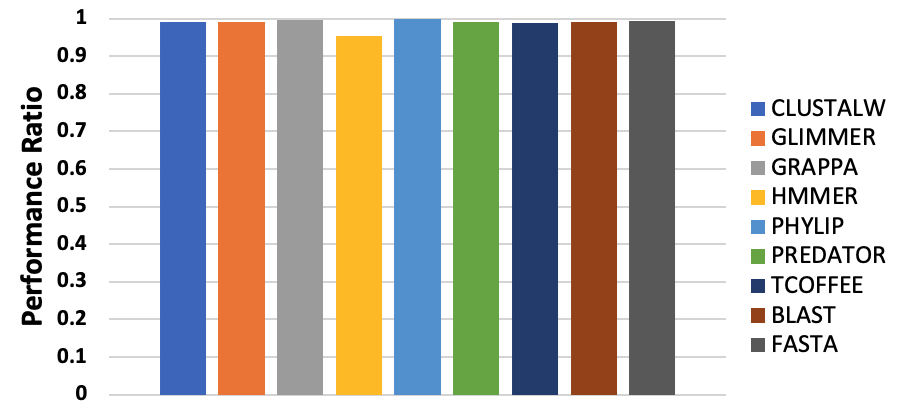
\includegraphics[width=\columnwidth]{Figures/perf_gap}
%    \end{center}
%    \caption{Performance ratio between virtual and bare metal for a set of life sciences workloads 
%    from BioPerf benchmark suite~\cite{1526013}. Higher is better. VMware ESXi 5.5 is used as the hypervisor.}
%    \label{fig:perf_gap}
%  \end{figure}

\subsection{HPC cloud resource allocation}
Virtualization brings new flexibility to HPC. With that flexibility, however, one must be careful to configure 
the cloud environment to simultaneously achieve both agility and high performance.
Although it is possible to create a single virtual cluster that spans an entire set of hosts
with one maximally sized VM per node, this approach misses the opportunity to enable several important 
virtualization benefits. Among these are the ability to support per-tenant or per-project software stacks as well 
as security and fault separation between the tenant workloads. In the more typical case, multiple virtual 
clusters should be hosted simultaneously on the physical cluster for isolation between tenants.

In a situation in which a tenant is using resources intensively, it might make most sense to assign 
a dedicated subset of hardware to the tenant and to configure VMs on those nodes appropriately. 
With two such tenants, one can either place their VMs on a non-overlapping set of nodes (Figure~\ref{fig:allocation1})
or place them on the same nodes, being careful to size their VMs to avoid any over-commitment (Figure~\ref{fig:allocation2}). 
%Typically, the size of each such VM is set to the number of cores available in each underlying physical CPU to take 
%advantage of the hardware NUMA topology. 
%This approach works well if the VMs are so heavily loaded that 
%few cycles are left unused on each node. However, it is often the case that such projects do not in actuality 
%show this degree of resource intensity. Although they might be very busy and resource constrained in some 
%time periods, they can also be less busy and even idle in other periods. In such cases, sizing VMs as 
%described--so that they partition the available physical cores--can lead to commensurate losses in 
%throughput because the idle CPUs serving one VM are not available to the other busy VM.
The major flaw with these approaches is that resources are statically partitioned and thus susceptible to under-utilization. 
Although tenants might be very busy in some 
time periods, they can also be less busy and even idle in other periods. In such cases, sizing VMs as 
described above can lead to commensurate losses in 
throughput because the idle resources serving one VM are not available to the other busy VM.

\begin{figure}
     \centering
     \begin{subfigure}[b]{0.45\textwidth}
         \centering
         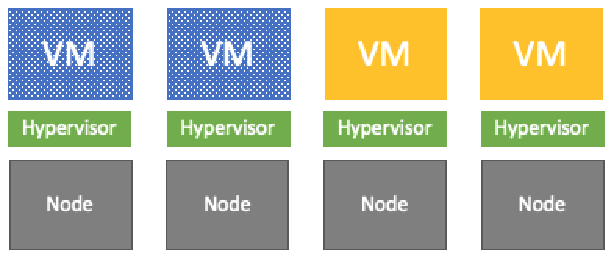
\includegraphics[width=\textwidth]{Figures/allocation1}
         \caption{Partition on non-overlapping nodes}
         \label{fig:allocation1}
     \end{subfigure}
     \hfill
     \begin{subfigure}[b]{0.45\textwidth}
         \centering
         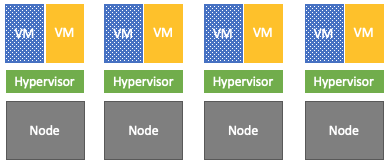
\includegraphics[width=\textwidth]{Figures/allocation2}
         \caption{Partition on same nodes}
         \label{fig:allocation2}
     \end{subfigure}
     \caption{Example of traditional static allocation with four hosts and two tenants. Gray VMs for one tenant and yellow VMs for the other.}
     \label{fig:static_allo}
\end{figure}

\subsection{Resource over-commitment}
The key to avoiding the above resource waste issue is resource over-commitment. In a 
virtualized environment, resource over-commitment means configuring VMs with more than the available 
physical resources. For example, on a host with 4 CPU cores and 8 GB memory, one could create and power on two VMs each 
with 4 virtual CPUs and 6 GB virtual memory. Resource over-commitment has been studied, but previous works did not optimize for HPC workloads 
and only considered CPU over-commitment~\cite{tran2019,Tesfatsion2018}.

CPU over-commitment is accommodated by multiplexing virtual 
CPUs onto the physical CPU cores. In the ESXi hypervisor, a share-based mechanism can be enabled  
in the scheduler so that each VM can get a different portion of the physical CPUs based on its configured shares, 
even in the case of over-commitment~\cite{vmware2013scheduler}. Furthermore, a work-conserving scheduler 
allows one VM to consume more than its fair CPU share if there are idle cycles from other VMs. 
Memory over-commitment, on the other hand, is more challenging since multiplexing is not 
applicable. It is achieved by a set of memory reclamation techniques, including transparent page sharing (TPS), 
ballooning, compression, and hypervisor swapping~\cite{Waldspurger:2002:MRM:844128.844146,banerjee2013memory}. These techniques differ in the incurred 
overhead and are individually controlled by the hypervisor based on system memory state.  



\section{Virtual Throughput Clusters}
\label{sec:vtc}
In the previous section we explained why naive resource allocation in virtual environments (Figure~\ref{fig:static_allo})
is sub-optimal for HPC workloads. This section will introduce our novel design that incorporates 
CPU and memory over-commitment for resource optimization. First, we start by introducing 
vHERO with CPU over-commitment. Then, we continue to discuss the 
inclusion of memory over-commitment which is much more challenging. Lastly, we complete the design 
with dynamic VM migration, which mitigates potential 
performance penalties from resource over-commitment. 

\subsection{vHERO with CPU over-commitment}
With a share-based CPU scheduler in the hypervisor, the allocation of CPU resource among VMs on a 
shared host does not entirely rely on the number of vCPUs, but also is affected by the configurable shares. 
This offers system admins the freedom to 
change VM vCPU count without worrying about impacting resource allocation. vHERO takes advantage of this 
flexibility and configures each tenant with the same amount of virtual CPUs as the physical CPUs 
on a node. In this way, each tenant can get access to all the CPUs inside the node, and consequently, if one tenant 
is not consuming its entire quota, the free CPU cycles can be used by other tenant(s). 
This approach can be easily scaled to a cluster by repeating the configuration on every 
single node. Then, each tenant is allocated a virtual cluster that consists of one VM per node. From the end user 
perspective, each tenant gets exclusive access to a dedicated cluster with security and fault isolation, and even better performance.  
Using the previous example of sharing four nodes between two tenants,  
vHERO is illustrated in Figure~\ref{fig:vtc}. In the experiment section later, we will demonstrate  
support of up to four tenants simultaneously on a single physical cluster with 4X CPU over-commitment.

\begin{figure}[!t]
   \begin{center}
       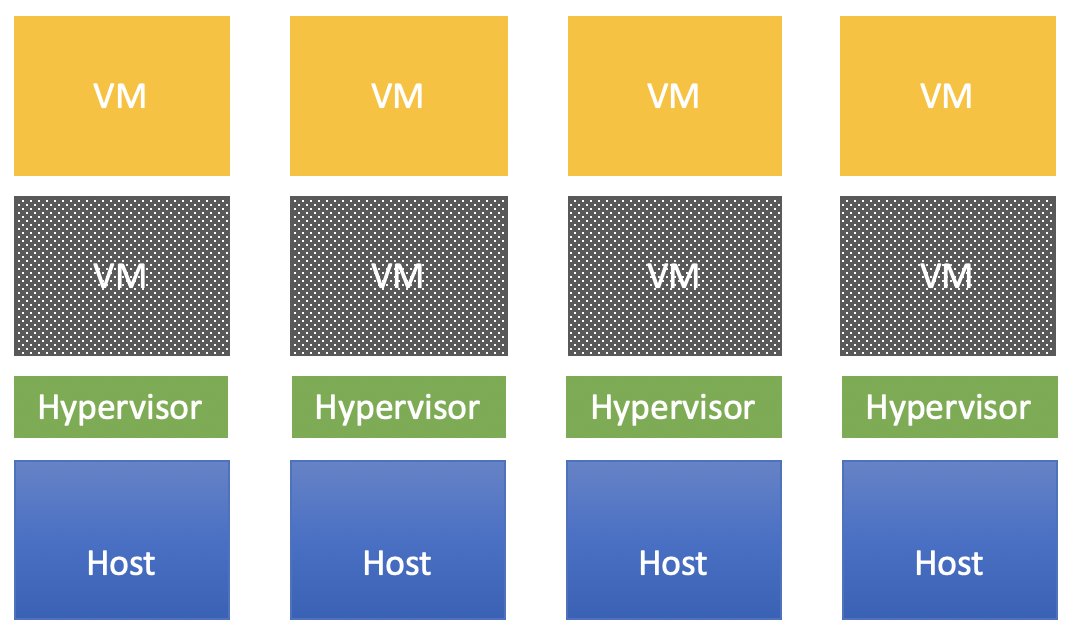
\includegraphics[width=\columnwidth]{Figures/allocation3}
   \end{center}
   \caption{Illustration of vHERO on four nodes for two tenants.}
   \label{fig:vtc}
 \end{figure}

\subsection{Adding memory over-commitment}
Similar to CPU over-commitment, memory can be configured in a way that the combined VM memory can be 
larger than the physical memory capacity. It is impossible, however, that all VMs actively access all configured 
memory beyond the physical capacity. This is mainly due to performance considerations. TPS, ballooning, and 
compression all have no guarantee to reclaim memory in a timely manner, and if all these techniques fail, 
hypervisor swapping will occur to swap out guest OS memory to disk, rendering unacceptable performance to 
the HPC workloads. Two questions that we address through our performance study are: 1) whether memory over-commitment 
can be practical; 2) how far can we go with active memory usage under memory over-commitment.

\subsection{Dynamic VM migration}
It's very restricting that while one can configure more VM memory, the VMs are not able to consume all of it 
at the same time. This constraint applies to every node in the cluster because if memory is over stressed on any 
node, the progress of the whole workload is impacted. 
Fortunately, vMotion can be applied to relax the constraint~\cite{infrastructure2006resource}. 
It is often the case that nodes in an HPC cluster have varying memory load~\cite{gupta2013improving}. While some nodes have memory contention 
between VMs, other nodes may have a decent amount of free memory. In such cases, vHERO with memory over-commitment 
is much more promising because VMs can be dynamically migrated based on load changes to  
spread the memory load evenly across the physical cluster. Ideally, none of the nodes will experience sustained memory pressure as long as 
the total active memory does not exceed the physical cluster memory capacity. This essentially relaxes the previous 
per-node constraint to a constraint per cluster, which has much more room for memory pressure tolerance. 

\section{Performance Evaluation}
\label{sec:eval}
Extensive experiments have been done to validate our design of VTC as well as evaluate 
its performance under various scenarios. This section covers our testbeds, experiment 
methodologies, performance tuning, results, and analysis. 

\subsection{Experiment setup}
The experiments are conducted in two phases. In the first phase, only CPU is over-committed 
to validate the design of VTC with over-commitment. In this phase, we used a cluster of 18 nodes (1 login node, 1 management node, and 16 compute nodes) to mimic a realistic HPC computing environment. Each node has dual 10-core Intel Xeon E5-2660 processor and 128 GB DDR4 memory. %, and 10 Gb Ethernet. 
The hypervisor used is VMware ESXi 6.5, OS is CentOS 7.3, and resource manager is TORQUE 6.1 with the default job scheduler. We use compute-intensive benchmarks from PolyBench/C 3.1 and BioPerf~\cite{1526013}. 
In the second phase, we evaluate the full-fledged VTC design with both CPU and memory over-commitment on another testbed with huge memory capacity for memory-intensive workloads. The second cluster has 1 login, 1 management, and 8 compute nodes. Each node has dual 16-core Intel Xeon Gold 6130 processor and 768 GB memory. %, and 10 Gb Ethernet. 
The hypervisor used is VMware ESXi 6.7, OS is CentOS 7.6, and resource manager is TORQUE 6.1 with the default job scheduler. We add memory-intensive benchmarks from HPCC~\cite{dongarra2004introduction}.

\subsection{CPU over-commitment}
For performance evaluation, each node is installed with two execution environments on two separate booting disks, that is, a native OS and an ESXi hypervisor. With the hypervisor, we further define three VTC scenarios: 1) one virtual cluster; 2) two virtual clusters; 3) four virtual clusters. The latter two scenarios have 2X and 4X CPU over-commitment, respectively. 
When comparing performance among different execution scenarios (including bare metal cluster), we run the same job stream which consists of 3248 jobs that are randomly sampled from the PolyBench and BioPerf suites, and the wall clock execution time is shown in Figure~\ref{fig:cpu_exe_time}.

\begin{figure}[!t]
   \begin{center}
       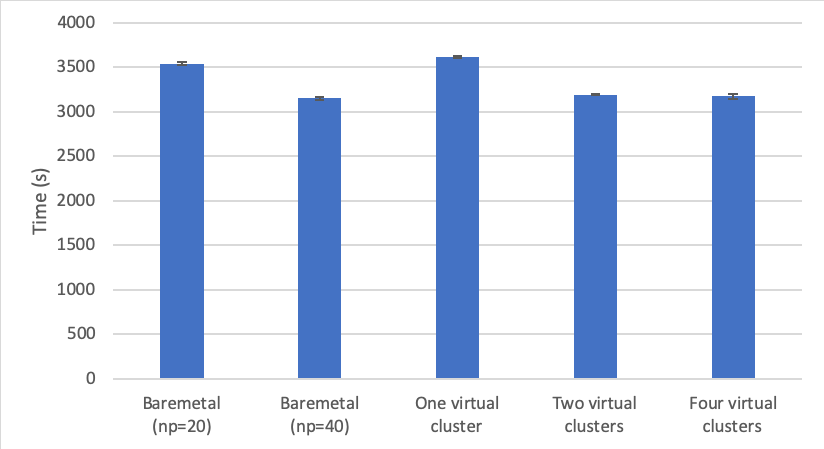
\includegraphics[width=\columnwidth]{Figures/cpu_exe_time}
   \end{center}
   \caption{Comparison of wall clock execution time for a job stream between bare metal and VTC with different CPU over-commitment ratios. Results are average of three runs.}
   \label{fig:cpu_exe_time}
 \end{figure}

Because each node in our testbed has 20 cores, in the first experiment we configured each TORQUE worker with 20 job slots. As reflected in Figure~\ref{fig:cpu_exe_time}, the execution with one virtual cluster is very close to that of bare metal (first column), with only a 2.2 percent overhead. Furthermore, when multiple virtual clusters are used with CPU over-commitment, the execution time is surprisingly shorter, implying an improved throughput despite the virtualization overhead. Through careful analysis, we identified that the throughput improvement can mainly be attributed to increased CPU utilization when more jobs are concurrently scheduled to execute. This has been verified by modifying each TORQUE worker in the bare-metal environment to use 40 job slots, after which the throughput is improved to the same level as the over-committed virtual environment. This can be seen in the second column of Figure~\ref{fig:cpu_exe_time}.

Besides execution time, another performance metric that we monitored is the total CPU utilization across the whole cluster. On the ESXi hypervisor, we used esxtop running on each compute node to sample CPU utilization of all VMs at 5-second intervals, and the results for one, two, and four virtual clusters are shown in Figure~\ref{fig:cpu_utilizations}. With two and four virtual clusters, the decreasing trend at the end is due to job completion. Clearly, CPU utilization is consistent with the job execution times in Figure~\ref{fig:cpu_exe_time}. For example, the lowest CPU utilization case--one virtual cluster--matches the longest job execution time. The higher CPU utilization with two and four virtual clusters is due to resource consolidation brought about by virtualization. That is, when multiple virtual clusters share a physical cluster, the CPU scheduler on each ESXi host has more jobs to schedule and is therefore able to make better scheduling decisions by taking advantage of Hyper-Threading and eliminating idle cycles. At the same time, improved utilization comes with better consistency, where the utilization with two and four virtual clusters is much smoother than in the single-cluster case.

\begin{figure}[!t]
   \begin{center}
       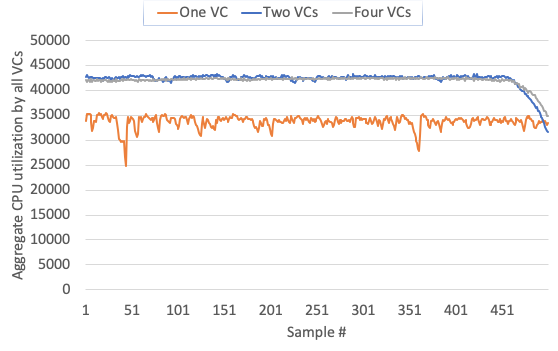
\includegraphics[width=\columnwidth]{Figures/cpu_utilizations}
   \end{center}
   \caption{Aggregate CPU utilization across 16 nodes at 5-seconds intervals.}
   \label{fig:cpu_utilizations}
   \vspace{-0.2in}
 \end{figure}

 In a production cloud environment, an important principle is fairness when multiple tenants are sharing the computing resources. We further examined the per-cluster CPU utilization in the multiple-cluster cases, and the case of four virtual clusters is shown in Figure~\ref{fig:per_cluster_utilization}. It is clear that the ESXi scheduler effectively maintains fairness so that each virtual cluster gets the same amount of CPU resources. The case of two virtual clusters is 
 the same thus not discussed. 


\begin{figure}[!t]
   \begin{center}
       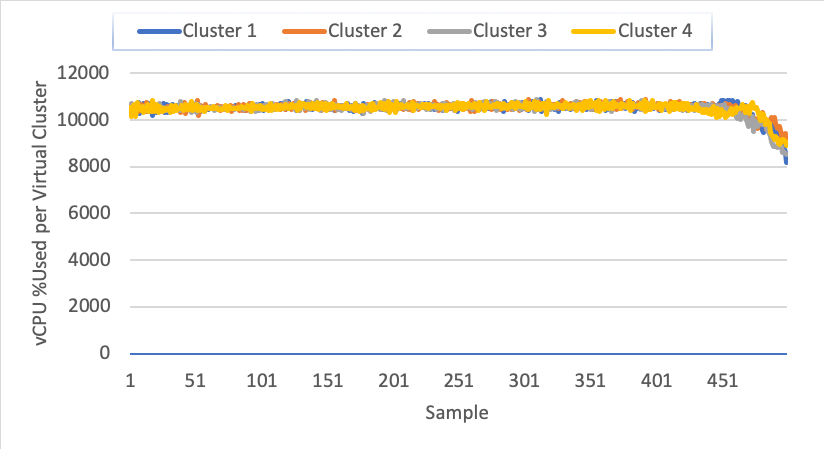
\includegraphics[width=\columnwidth]{Figures/per_cluster_utilization}
   \end{center}
   \caption{Plot of CPU utilization per virtual cluster at 5-seconds intervals for fairness check.}
   \label{fig:per_cluster_utilization}
   \vspace{-0.2in}
 \end{figure}

\subsection{CPU over-commitment with shares}
In addition to the option of equally sharing resources, the proportional, share-based scheduler of the ESXi hypervisor offers a very useful degree of flexibility. This subsection continues the CPU over-commitment study by configuring virtual clusters with different shares, to demonstrate the capability of creating a multi-tenant environment with quality-of-service guarantees. 

With the use of CPU shares, each VM can be given a particular guaranteed share of CPU resources. When there are multiple VMs running on an ESXi host, the ESXi scheduler allocates CPU based on the ratio of shares among all the running VMs. This feature extends to a virtualized HPC cloud. Specifically, each user or group can be given an appropriate share of the physical system when their virtual cluster is allocated. In this experiment, we focus on the case of four virtual clusters and set the shares ratio among the four VMs as 2:1:1:1 on every compute node. The CPU utilization is shown in Figure~\ref{fig:share_utilization}. Clearly, the CPU utilization ratio among the virtual clusters is the same as the specified shares ratio. Another important observation is that the aggregate CPU utilization across 4 virtual clusters is the same as previous no-shares case as depicted in Figure~\ref{fig:cpu_utilizations}.


\begin{figure}[!t]
   \begin{center}
       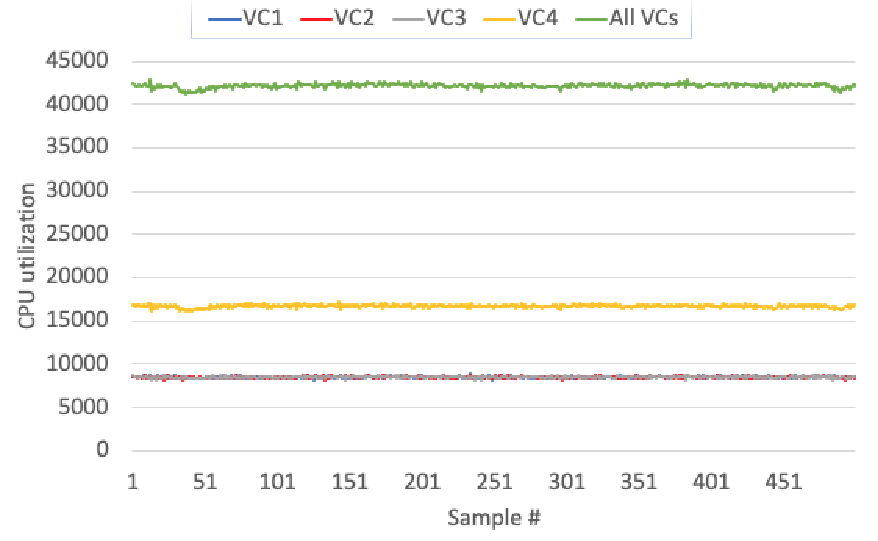
\includegraphics[width=\columnwidth]{Figures/share_utilization}
   \end{center}
   \caption{CPU utilization for four virtual clusters with 2:1:1:1 CPU shares. Utilization is sampled at 5-second intervals.}
   \label{fig:share_utilization}
 \end{figure}

\subsection{CPU + memory over-commitment}
Given that memory over-commitment is more challenging, we only test two virtual clusters with 2X CPU and memory over-commitment. vSphere Dynamic Resource Scheduler (DRS) is used to dynamically control VM migration for load balancing~\cite{infrastructure2006resource}. Considering the VM migration cost, we decided to use four quarter-size VMs to replace the single full-size VM on each node for each tenant. As a result, each tenant in this experiment gets a virtual cluster of 32 VMs across the 8 node cluster. 

To stress the system memory, we added benchmarks from HPCC. For all these HPCC benchmarks, a problem size of 53664 is chosen to have the memory consumption ranging from 16 GB to 22 GB per job instance. All the benchmarks are run with a single threaded process to mimic throughput workloads. 
To model a real HPC tenant, we specify the job arrival time to follow a Gamma distribution based on the study of several production HPC systems~\cite{lublin2003workload}.  
The resulted mean job inter-arrival time is 20.88 seconds
%The Gamma distribution has a shape parameter of 10.23 and scale parameter of 0.49. With those parameters, the mean job inter-arrival time is 10.23 / 0.49 = 20.88 seconds. 
%Also, all job sequences are shuffled to generate randomized job streams. Then, two execution scenarios are designed to represent different workload patterns. 

Two execution scenarios are designed to represent different workload patterns. In the first scenario, 1600 HPCC jobs (memory-intensive) are submitted to the first virtual cluster all at the beginning, while 1500 BioPerf jobs (memory-light) arrive at the second virtual cluster following the above Gamma distribution. The number of jobs are determined to let the two virtual clusters finish at roughly the same time. In the first virtual cluster, all the job slots will be consumed immediately and the jobs will maximize their utilization of the cluster's CPU and memory resources. In the second cluster, CPU and memory load will gradually build up. 
We make the second scenario more demanding by running two HPCC streams of 1600 jobs following the Gamma distribution. 
%Were all job slots being used, the active memory consumption would largely exceed the physical memory capacity. 
It's demanding because, even if each job only consumes 16 GB memory, 64 job instances on each node will require 64 * 16 GB = 1024 GB, which is much larger than the node capacity. It is well understood that ESXi cannot support that kind of memory over-usage. But, it is still worthwhile to explore in the realistic case where jobs randomly come and go, whether DRS can collaborate with ESXi memory reclamation techniques to accommodate this usage pattern. 

In each scenario, we run w/ and w/o DRS and measure two metrics: 1) wall clock time (WCT), i.e., the elapsed time from the start of job submission to the completion of the last job; 2) cumulative job execution time (CJET), i.e., the cumulative sum of all job instances' execution time. 

%The first metric is a measure of the system throughput, and the second metric indicates system efficiency. 
The results in scenario 1 are plotted in Figure~\ref{fig:memory_scenario1}. As the figures suggest, while VTC successfully supported 2X CPU and memory over-commitment regardless of DRS, DRS reduces HPCC's WCT by 11.1\%, which is a great improvement in throughput. 
The reason why DRS doesn't reduce BioPerf's WCT is that BioPerf jobs strictly follow the Gamma distribution in job arrivals.
But as we can see in Figure~\ref{fig:memory_cjet}, DRS reduces BioPerf's CJET by 18.4\%, making room available for more jobs. HPCC's CJET slightly increases with DRS and it indicates that DRS can cause minimal overhead to individual jobs due to telemetry sampling and VM migration. 
%, but increases HPCC CJET by 1.1\%, which is negligible. 
The number of VM migrations in each run is in the range of 30-40. It's interesting to notice that all migrations happened to the BioPerf VMs, which is because BioPerf VMs have smaller memory footprint and are lighter to migrate.

\begin{figure}
     \centering
     \begin{subfigure}[b]{0.45\textwidth}
         \centering
         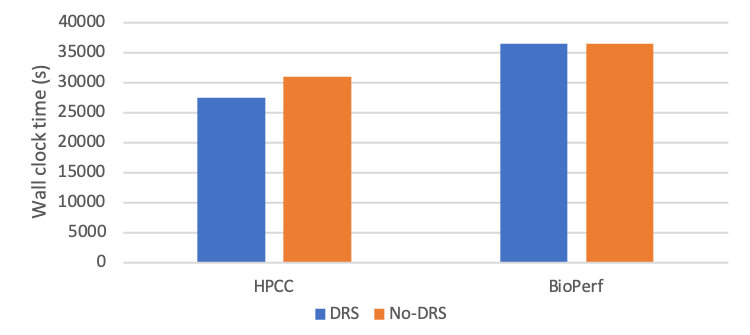
\includegraphics[width=\textwidth]{Figures/memory_wct}
         \caption{Wall clock time}
         \label{fig:memory_wct}
     \end{subfigure}
     \hfill
     \begin{subfigure}[b]{0.45\textwidth}
         \centering
         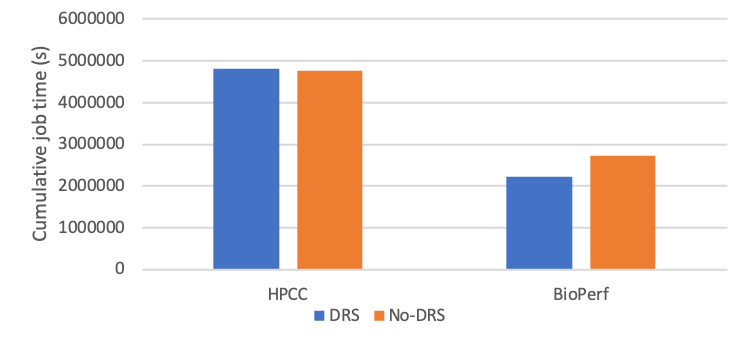
\includegraphics[width=\textwidth]{Figures/memory_cjet}
         \caption{Cumulative job execution time}
         \label{fig:memory_cjet}
     \end{subfigure}
     \caption{Comparison between DRS enabled and DRS disabled for VTC with 2X CPU and memory over-commitment. Workloads are from scenario 1. }
     \label{fig:memory_scenario1}
\end{figure}

As mentioned above, the second scenario is much more demanding because HPCC jobs can potentially consume all the configured VM memory. It's not a surprise the cluster is not able to finish two simultaneous streams of HPCC jobs, regardless of whether DRS is used. The guest OS encountered CPU soft lockup errors when hypervisor swapping occurs and when swapping is not responsive enough. Our analysis identified HPL (one benchmark in the HPCC suite) jobs as the bottleneck. Each HPL job needs more than 3 hours to finish, and once enough HPL instances accumulate on any node, the hypervisor is not able to handle their excessive memory requirements. Therefore, we decided to remove HPL from the job stream. After this change, we see that two HPCC streams can finish when DRS is on. Without DRS, the same failure occurs. Clearly, this demonstrates the effectiveness of DRS in load balancing and mitigating memory pressure. 

Though HPCC VMs are heavier to migrate, on average 67 VM migrations occurred per run, due to the extreme memory stress. Naturally, one may concern that the large number of migrations could introduce jitters to the running workloads. To quantify that, we collect the execution time distribution among all instances for each benchmark. It turns out that the execution time is quite consistent. For example, the histogram for RandomAccess (another benchmark in the HPCC suite) is shown in Figure~\ref{fig:ra_histogram}.

\begin{figure}[!t]
   \begin{center}
       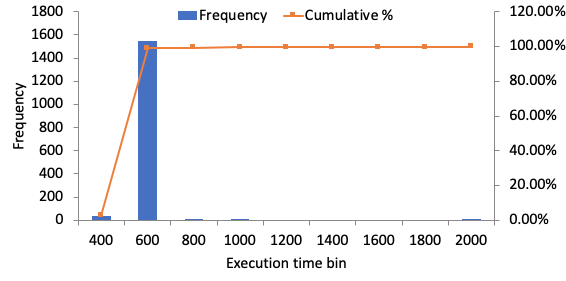
\includegraphics[width=\columnwidth]{Figures/ra_histogram}
   \end{center}
   \caption{Histogram of individual RandomAccess job execution time from both virtual clusters.}
   \label{fig:ra_histogram}
 \end{figure}






% \section{Related Work}
% \label{sec:related}
% %Extreme-scale computing presents some unique challenges to fault tolerance as faults are no longer 
%an exceptional event \cite{ferreira_sc_2011}. 
Rollback and recovery is the predominate mechanism to achieve fault
tolerance in current HPC environments. In the most general form, rollback and recovery 
involves the periodic saving of the current system state, with the anticipation that
in the case of a failure, computation can be restarted from the most recently saved state \cite{Elnozahy:02:Survey}. %The identification of an error, before or during a checkpoint,
%requires that the application rollback to the previously completed checkpoint. 
Coordinated checkpointing is a popular approach for
its ease of implementation.
%Specifically, all processes
%coordinate with one another to produce individual states that satisfy the ``happens before"
%communication relationship \cite{chandy_trans_1972}, which is proved to provide a consistent global state.
%Essentially, the algorithm provides a method for all processes involved to stop operation ``at the same
%time" and transfer their system state to a stable storage. 
%The major benefit of coordinated
%checkpointing stems from its simplicity and ease of implementation. 
Its major drawback, however, is the
lack of scalability, as it requires global coordination
\cite{elnozahy_dsc_2004,riesen_sandia_2010}.
%hargrove2006berkeley}.


In uncoordinated checkpointing, processes record their states independently and postpone creating a 
globally consistent view until the recovery phase. The major advantage is the reduced overhead during fault free operation. However, the scheme requires that
each process maintains multiple checkpoints and message logs, necessary to construct a consistent 
state during recovery. It can also suffer the well-known domino effect 
 \cite{randell_domino_effect}. One hybrid approach, known as communication induced 
checkpointing, aims at reducing coordination overhead \cite{alvisi_ftc_1999}. The approach, however, may 
cause processes to store useless states. To address this 
shortcoming, ``forced checkpoints" have been proposed \cite{helary_rds_1997}. This approach, however,  may lead to unpredictable
checkpointing rates. Although well-explored, uncoordinated checkpointing has not been widely adopted
in HPC environments, due to its dependency on applications \cite{guermouche_2011_ipdps}.


One of the largest overheads in any checkpointing process is the time necessary to write the checkpointing 
to stable storage. Incremental checkpointing attempts
to address this by only writing the changes since previous checkpoint \cite{Agarwal:04:Adaptive,elnozahy_1992_manetho,li_trans_1994}. %This
%can be achieved using dirty-bit page flags \cite{plank_ftcs_1994,elnozahy_1992_manetho}. Hash based incremental checkpointing, on the other
%hand, makes use of hashes to detect changes \cite{nam_ftc_1997,Agarwal:04:Adaptive}. 
Another proposed scheme, known as in-memory checkpointing, minimizes the overhead of disk access~\cite{zheng_2004_ftccharm}.
%offloads the checkpointing process to a secondary task and only writes incremental checkpoints \cite{li_trans_1994}.
The main concern of these techniques is the increase in
memory requirement to support the simultaneous execution of the checkpointing and the application. It has been suggested that nodes in extreme-scale systems should be configured with fast local storage~\cite{doe_ascr_exascale_2011}. 
%, which
%improves the performance of checkpointing \cite{doe_ascr_exascale_2011}. 
Multi-level checkpointing, which consists of
writing checkpoints to multiple storage targets, can benefit from such a strategy \cite{Moody:10:SCR}. This,
however, may lead to increased failure rates of individual nodes and complicate the checkpoint writing process.
%Furthermore, it may complicate the checkpoint writing process and requires that the system track the
%current location of all process's checkpoints.


Our work is based on process replication, or state machine replication, which has long been used to provide fault tolerance in distributed and mission critical systems\cite{schneider_1990_tutorial}. %Replication can be used to detect and correct system failures that are otherwise undetectable,
%such as silent data corruption and Byzantine faults \cite{fiala_2012_sdc}. 
Recently, replication has been proposed as a
viable alternative to checkpointing in HPC \cite{ferreira_sc_2011,Cappello:09:Fault,fiala_2012_sdc}. 
In addition, full and partial
replication have also been used to augment existing checkpointing techniques, and to guard
against silent data corruption \cite{stearly_2012_partial,elliott_2012_cpr}.% There are several different implementations of
%replication in the widely used MPI library, each with their different tradeoffs and overheads. The
%overhead can be negligible or up to 70\% depending upon the communication patterns of the
%application \cite{engelmann2011redundant}. %Moreover, replication alone is not enough to guarantee fault tolerance since
%it is possible that all nodes executing a given process could fail simultaneously, thus
%replication is typically paired with some form of checkpointing. 
The most relevant works to ours is redundant multi-threading (RMT) whereby one leading thread of execution is running ahead of trailing threads \cite{reinhardt2000transient,Wadden:2014:RDE:2665671.2665686}. However, our approach is different in that it tunes the execution rates of the leading and trailing threads in a finer grain, in order to achieve a ``parameterized" trade-off between completion time and energy consumption. Further, we take advantage of the idle time during failure recovery and ``leap" the trailing threads to achieve forward progress%, largely improving performance in terms of both completion time and energy consumption. 
. This differs from RMT, of which the ``leaping" of the trailing thread results in extra overhead.
%To the best of our knowledge,
%Lazy Shadowing is the first attempt to explore a state-machine replication based framework
%that achieves a fine-grained tradeoff between time and hardware redundancy while meeting resilience and
%power requirements.


\section{Conclusion}
\label{sec:conslusion}
%Current fault-tolerance approaches rely exclusively on either time or hardware redundancy for recovery. Rollback recovery  exploits time redundancy but can incur significant delay and high energy cost. On the other hand, process replication relies on hardware redundancy and requires a significant increase in resources and  power consumption.

In this paper, we propose Rejuvenating Shadows as a novel power-aware fault tolerance model, which guarantees forward progress, maintains consistent level of resilience, and minimizes implementation complexity and runtime overhead. Empirical experiments demonstrated that the Rejuvenating Shadows model outperforms in-memory checkpointing/restart in both execution time and resource utilization, especially in failure-prone environments.

Leaping induced by failure has proven to be critical in reducing the divergence between a main and its shadow, 
%with respect to workload execution.
%Consequently, the time to recover from subsequent failures is reduced significantly. 
thus reducing the recovery time for subsequent failures. Consequently, the time to recover from a failure increases with failure intervals.  
Based on this observation, a proactive approach is to ``force" leaping when the divergence between a main and its shadow exceeds a specified threshold. 
In our future work, we will further study this approach to determine what behavior triggers forced leaping in order to optimize the average recovery time. 

%we will study forcing the shadDuring experimentation we noticed the problem that recovery time in Rejuvenating Shadows can become substantial when the failure interval is large (Figure~\ref{fig:single_failure}). To deal with this issue, we are studying the idea of ``forced leaping", which borrows the idea from periodic checkpointing and forces a leaping whenever failure has been absent for a long time, in order to reduce the divergence between mains and shadows. Optimal intervals for forced leaping will be explored to balance between runtime overhead and failure recovery overhead. 

%In the future we plan to explore the integration with fault prediction techniques and the viability of dynamic and partial shadowing for platforms where nodes exhibit different ``health" status, e.g., some nodes may be more reliable while others are more likely to fail~\cite{gainaru2012fault}. 
%With this taken into account, we can apply dynamic scheduling of shadows only for mains that are likely to fail, to further reduce the resource requirement. 
%Another future direction is to study complier-assisted program slicing for fault detection. Specifically, slices that are fraction of their mains can run lazily as shadows and provide fault detection capability with reasonable coverage. 





%% Acknowledgments
% \begin{acks}                            %% acks environment is optional
%   The authors would like to thank Onur Celebioglu for providing the first testbed in 
%   the Dell EMC HPC and AI Innovation Lab, and to thank Justin King and Shree Das for providing and 
%   setting up the second testbed. The authors also appreciate the help from Yury Baskakov, 
%   Mark Achtemichuk, and Zhelong Pan on experiment design and results analysis. 

% \end{acks}


%% Bibliography
\bibliography{main}
                

\end{document}
